\chapter{Непрерывные функции от нескольких переменных}


\section{Непрерывные отображения}

\begin{definition}
Пусть $X \subseteq \mathbb{R}^n$, отображение $F:X \to \mathbb{R}^m$ называется \textit{непрерывным в точке} $\m{x}_0 \in X$, если для для каждой окрестности $\mathscr{U}'$ точки $F(\m{x}_0) \in \mathbb{R}^m$ существует такая окрестность $\mathscr{U}(\m{x}_0)$ в $X$, что $F(\mathscr{U}(\m{x}_0)) \subseteq \mathscr{U}'(F(\m{x}_0))$. Отображение $F$ называется \textit{непрерывным в $\mathbb{R}^n$} (или просто непрерывным), если оно непрерывно в каждой точке пространства $\mathbb{R}^n.$
\end{definition}

Это же определение можно переформулировать и таким образом:

\begin{definition}
    Отображение $F:X \to \mathbb{R}^m$ непрерывно в точке $\m{x}_0$, если для любого шара $B(F(\m{x}_0), r) \subseteq \mathbb{R}^m$ всегда можно найти такой открытый в $X$ шар $B(\m{x}_0, \delta) \subseteq X$, что $F(B(\m{x}_0, \delta)) \subseteq B(F(\m{x}_0), r)$.
\end{definition}

Можно ещё вот так сказать:

\begin{definition}\label{reform_of_cont}
    Для того, чтобы отображение $F:X \to \mathbb{R}^m$ было непрерывно в точке $\m{x}_0 \in X$, необходимо и достаточно, чтобы для всякого $\varepsilon>0$ существовал такой $\delta >0$, что из $\|\m{x} - \m{x}_0\|<\delta$ следует $\| F(\m{x}) - F(\m{x}_0) \|<\varepsilon$.
\end{definition}

\begin{figure}[h!]
    \centering
    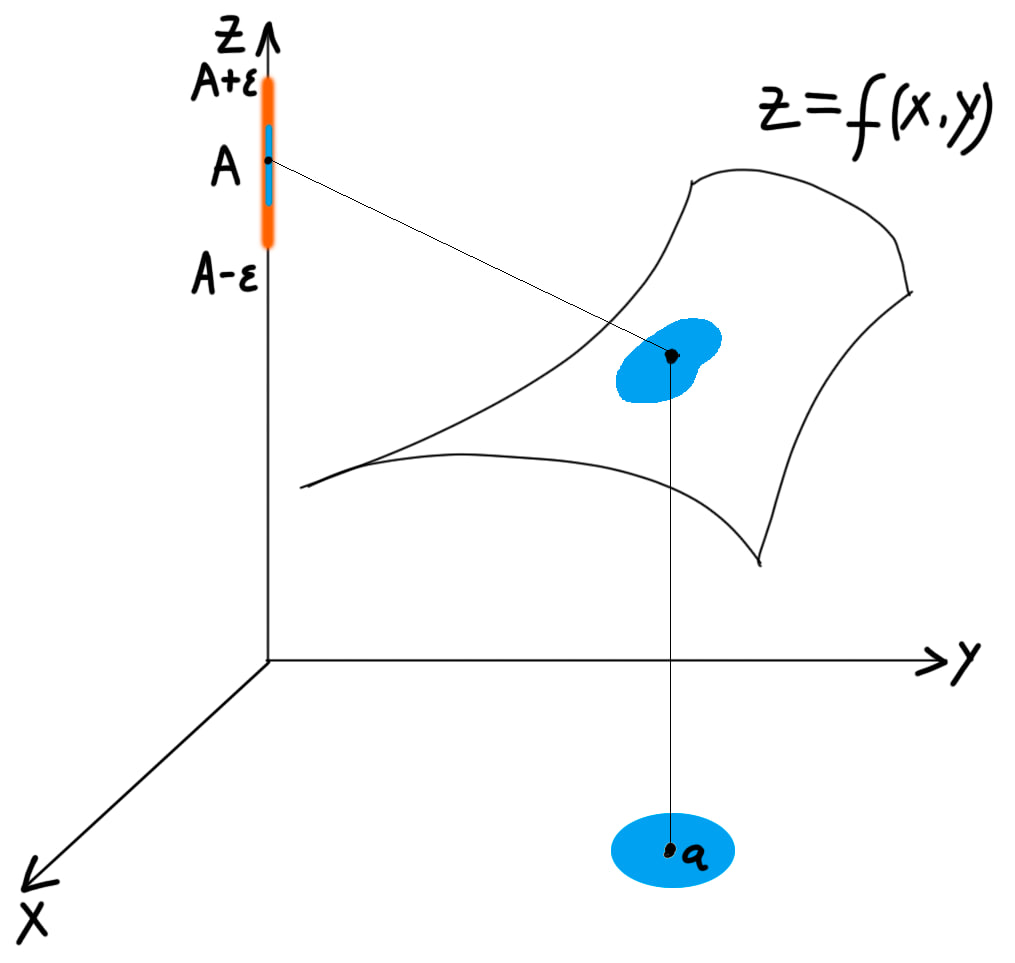
\includegraphics[scale=0.5]{images/continous3.jpg}
    \caption{График отображения $f: \mathbb{R}^2 \to \mathbb{R}$ есть некоторая поверхность в $\mathbb{R}^3$. Нужно понимать, что мы горизонтальную плоскость отображаем в вертикальную прямую. Здесь показано, почему в точке $\m{a}\in \mathbb{R}^2$ это отображение непрерывно, $f(\m{a}) = A$. Какой бы оранжевый шар $\textcolor{orange}{B(A, \varepsilon)} \subseteq \mathbb{R}$ мы не взяли, можно найти синий шар $\textcolor{blue}{B(\m{a},r)} \in \mathbb{R}^2$ такой, что его образ $f( \textcolor{blue}{B(\m{a}, r)} )$ в вертикальной прямой (синяя полоска в оранжевом отрезке) будет целиком содержаться в этом оранжевом шаре.}
    \label{fig:enter-label}
\end{figure}


\begin{remark}\label{not_continous}
    Тогда если $f(x)$ не является непрерывным в точке $x_0$, то какой бы шар $B(x_0, \delta) \subseteq E$ мы не выбрали, всегда можно найти такой шар $B(f(x_0),r)$, что $f(x) \notin B(f(x_0),r)$ для каких-то $x \in B(x_0, \delta).$
\end{remark}



\begin{theorem}\label{preimage_of_open}
 Отображение $F:X \to \mathbb{R}^m$ непрерывно тогда и только тогда, когда прообраз любого открытого в $\mathbb{R}^m$ открыт в $X.$
\end{theorem}
\begin{proof}~

(1) Пусть $f:E \to E'$ непрерывно. Возьмём открытое $\mathscr{U}' \subseteq E'$ и покажем, что $\mathscr{U}:=f^{-1}(\mathscr{U'})$ открыто в $E$. Пусть $x \in \mathscr{U}$, тогда $f(x) = x' \in \mathscr{U}'$, так как $\mathscr{U}'$ -- открыто в $E'$, то найдётся шар $B'(x',r') \subseteq \mathscr{U}'$. Так как шар $B'(x',r')$ есть открытая окрестность точки $x'$ и по предположению $f$ непрерывна и в точке $x \in E$, значит, найдётся такой шар $B(x,r) \subseteq E$ такой, что $f(B(x,r)) \subseteq B'(x',r')$. 

Таким образом, мы имеем $f(B(x,r)) \subseteq B'(x',r') \subseteq \mathscr{U}' .$ С другой стороны, если $A'\subseteq B' \subseteq E'$, то ясно, что $f^{-1}(A') \subseteq f^{-1}(B')$. Действительно, по определению прообраза
    \[
     f^{-1}(A'):= \{x \in X\, |\, f(x) \in A' \subseteq B'\} \Longrightarrow f^{-1}(A') \subseteq f^{-1}(B').
    \]

 Итак, мы получили, что $f(B(x,r)) \subseteq B'(x',r') \subseteq \mathscr{U}'$, тогда
 \[
  f(B(x,r)) \subseteq \mathscr{U}' \Longleftrightarrow f^{-1}(f(B(x,r))) \subseteq f^{-1}(\mathscr{U}')  \Longleftrightarrow B(x,r) \subseteq \mathscr{U},
 \]
 \ie для любого $x \in \mathscr{U}$ мы нашли шар $B(x,r)$, который целиком находится в $\mathscr{U}$, а это и означает, что $\mathscr{U}$ открыто.

(2) Пусть прообраз любого открытого есть открытое множество в $E.$ Пусть $\mathscr{U}'$ -- открытое в $E'$. Аксиома выбора позволяет нам выбрать точку $x' \in \mathscr{U}'$. Тогда для произвольно выбранной точки $x'$ существует такой открытый шар $B'(x',r')$, что $B'(x',r') \subseteq \mathscr{U}'.$

Пусть $f(x) = x'$, \ie $x \in f^{-1}(B'(x',r'))$. По предположению $f^{-1}(B'(x',r'))$ открыто в $E$. Это значит, что для любой выбранной точки $y \in f^{-1}(B'(x',r'))$ можно найти такой открытый шар $B(y,r)$, что $B(y,r) \subseteq f^{-1}(B'(x',r'))$. В частности, $B(x,r) \subseteq f^{-1}(B'(x',r'))$ 

Вспоминая, что если $A \subseteq B$, то и $f(A) \subseteq f(B)$. Тогда получаем 
\[
  B(x,r) \subseteq f^{-1}(B'(x',r')) \Longrightarrow f(B(x,r)) \subseteq f(f^{-1}(B'(x',r'))) \subseteq B'(x',r'),
\]
\ie для любого открытого шара $B'(x',r')$, где $x' = f(x)$, мы нашли такой открытый шар $B(x,r)$, что $f(B(x,r)) \subseteq B'(x',r')$, но это и означает непрерывность.
\end{proof}

\begin{corollary}
    Отображение $f:E \to E'$ -- непрерывно в точке $x$, тогда и только тогда, когда прообраз любого открытого шара $B(f(x),r) \subseteq E'$ -- открытое множество в $E$
\end{corollary}
\begin{proof}
    Это сразу следует из предыдущей теоремы и леммы \ref{union_and_cap_of_open}.
\end{proof}

\begin{theorem}\label{comp_of_continous}
    Пусть $E,E,E''$ -- метрические пространства и пусть $f:E \to E'$, $g:E' \to E''$ -- отображения. Если $f$ непрерывно в точке $x_0$ и $g$ непрерывно в $f(x_0)$, то $h = g \circ f$ непрерывно в точке $x_0.$ Если $f$ непрерывно в $E$ и $g$ непрерывно в $E'$, то $h$ непрерывно в $E.$
\end{theorem}
 \begin{proof}
     Второе утверждение, очевидно, следует из первого. Пусть $\mathscr{U}''$ -- окрестность точки $h(x_0) =  g(f(x_0))$. Тогда из предположения о непрерывности и Теоремы \ref{preimage_of_open} следует, что $\mathscr{U}':=g^{-1}(\mathscr{U}'')$ -- открытое множество в $E'$, содержащее точку $f(x_0)$. Далее, так как $f$ непрерывно, то по теореме \ref{cap_of_intervals}, прообраз $\mathscr{U}:=f^{-1}(\mathscr{U}')$ -- открытое множество, содержащее точку $x_0$. Таким образом, $h^{-1}(\mathscr{U}'') = \mathscr{U}$ открытое, тогда по теореме \ref{preimage_of_open}, $h$ непрерывно в точке $x_0$, что и завершает доказательство. 
 \end{proof}


\begin{corollary}\label{restriction}
    Если $f$ -- отображение метрического пространства $E$ в метрическое пространство $E'$, непрерывное в точке $x_0$, и $A \subseteq E$, $A \ni x_0$, то сужение $f|_A:=f \circ \mathrm{in}_A$ также непрерывно в $x_0,$ где $\mathrm{in}_A:A \hookrightarrow E$ -- вложение.
\end{corollary}
\begin{proof}
    На самом деле, $f$ непрерывно в $x_0$ по условию, а $\mathrm{in}_A$ непрерывно в любой точке $a \in A$, тогда из предыдущей теоремы и следует утверждение.
\end{proof}

 \begin{remark}\label{+infty}
    Пусть $E = \overline{\mathbb{R}}$ -- расширенная прямая, рассмотрим выражение $$\lim_{x \to +\infty, x \in \mathbb{{R}}}f(x) = a',$$ где $f:\mathbb{R} \to E' $ -- некоторое отображение. Мы знаем, что $B(+\infty, \delta) = (\frac{1-\delta}{\delta}, \infty]$. Тогда непрерывность в точке $+\infty$ означает, что для любого $r >0$ найдётся такая $\delta>0$, что $f((\frac{1-\delta}{\delta}, \infty]) \subseteq B(a',r)$. Другими словами, для любого шара $B(a',r)$ найдётся такое число $\alpha \in \mathbb{R}$, что $f(\beta) \in B(a',r)$ для всех $\beta > \alpha.$
\end{remark}





\begin{lemma}\label{preimage_of_closed}
    Отображение $f:E \to E'$ между метрическими пространствами непрерывно тогда и только тогда, когда прообраз любого замкнутого множества в $E'$ есть замкнутое множество в $E.$
\end{lemma}

\begin{proof}
    Пусть $F'$ -- замкнутое подмножество в $E'$, тогда $\mathscr{U}': = E'\setminus F'$ -- открыто в $E'$ и $E' = F' \cup \mathscr{U}'$, $F' \cap \mathscr{U}' = \varnothing$. Далее, ясно что $f^{-1}(F') \cap f^{-1}(\mathscr{U}') = \varnothing$ и $E = f^{-1}(F') \cap f^{-1}(\mathscr{U}')$. Тогда согласно Теореме \ref{preimage_of_open}, $f$ -- непрерывно если и только если $f^{-1}(\mathscr{U}')$ -- открыто в $E$, но тогда $f^{-1}(F') = E \setminus \mathscr{U}'$ замкнуто тогда и только тогда, когда $f^{-1}(\mathscr{U}')$ -- открыто. Это завершает доказательство.
\end{proof}



\section{Пределы}

Пусть $(\m{V}, \|\cdot\|_1)$ -- нормированное пространство, пусть $\mathcal{S} \subseteq \m{V}$ -- некоторое его подмножество, пусть $\m{v}_0$ -- точка прикосновения для $\mathcal{S}$, \ie $\m{v}_0 \in \overline{\mathcal{S}}$, и пусть $F:\mathcal{S} \to \m{W}$ некоторое отображение в нормированное пространство $(\m{W}, \|\cdot\|_2).$

\begin{definition}\label{the_main_def_of_limit}
Пусть $\m{v}_0 \notin \mathcal{S}$. Мы будем говорить, что $F(x)$ \textit{имеет предел $\m{w}_0 \in \m{W}$ при $\m{v} \in \mathcal{S}$, стремящемся к $\m{v}_0$ (или $\m{w}_0$ есть предел отображения $F$ в точке $\m{v}_0\in \overline{\mathcal{S}}$ по множеству $\mathcal{S}$}), если отображение $\overline{F}:\mathcal{S} \cup \{\m{v}_0\} \to W$, определённое условиями
    \[
     \overline{F}(\m{v}) := \begin{cases}
         F(\m{v}), & \m{v} \in \mathcal{S}, \\
         \m{w}_0, & \m{v} = \m{v}_0,
     \end{cases}
    \]
    непрерывно в точке $\m{v}_0$.
\end{definition}

В этом случае, мы пишем
\[
 \m{w}_0 := \lim_{\m{v}\to \m{v}_0, \m{v} \in \mathcal{S}} F(x).
\]

\begin{mydanger}{\bf{!}}
Если $\m{v}_0 \in \mathcal{S}$, то мы пользуемся той же терминологией и теми же обозначениями как и в случае, когда отображение $F$ непрерывно в точке $\m{v}_0$, причём $\m{w}_0:=F(\m{v}_0).$
\end{mydanger}

Вспомнив определение непрерывности и открытого множества в подмножестве, и точки прикосновения, определение предела можно переформулировать следующими двумя эквивалентными способами:

\begin{definition}
 $\lim_{\m{v}\to \m{v}_0, \m{v} \in \mathcal{S}} F(x) = \m{w}_0$ эквивалентно тому, что для любого шара $B(\m{w}_0,r) \subseteq \m{W}$ найдётся такой шар $B(\m{v}_0,\delta)$, что $F(B(\m{v}_0,\delta)\cap \mathcal{S}) \subseteq B(\m{w}_0,r)$.
\end{definition}
\begin{mydanger}{\bf{!}}
    Так как $\m{v}_0$ -- точка прикосновения, то множество $B(\m{v}_0,\delta) \cap \mathcal{S}$ никогда не пусто для любого $\delta >0$, а также октрыто в $\mathcal{S}.$
\end{mydanger}

\begin{definition}\label{def_for_cont_via_d-e}
$\lim_{\m{v}\to \m{v}_0, \m{v} \in \mathcal{S}} F(x) = \m{w}_0$ эквивалентно тому, что для каждого $\varepsilon>0$ можно найти такое $\delta >0$, что из $\m{v} \in \mathcal{S}$ и $\|\m{v} - \m{v}_0\|_1 <\delta$ следует $\|F(\m{v}) - \m{w}_0\|_2<\varepsilon.$
\end{definition}

\begin{proposition}
    Отображение может иметь лишь один предел по множеству $A$ в данной точке $a \in \overline{A}.$
\end{proposition}
\begin{proof}
    Пусть  $\lim_{x \to a, x \in A}f(x) = a'$ и  $\lim_{x \to a, x \in A}f(x) = b'$, при этом $a' \ne b'$. Тогда, согласно Определению \ref{def_for_cont_via_d-e}, 
 \begin{enumerate}
     \item  $\lim_{x \to a, x \in A}f(x) = a'$ означает, что для любого $\varepsilon >0$ можно найти такое $\delta_1 >0$, что из $x \in A$ и $\|x-a\|_1<\delta_1$ следует $\|a'-f(x)\|_2<\varepsilon$
     \item $\lim_{x \to a, x \in A}f(x) = b'$ означает, что для того же $\varepsilon >0$ можно найти такое $\delta_2 >0$, что из $x \in A$ и $\|x-a\|_1<\delta_2$ следует $\|b'-f(x)\|_2<\varepsilon$.
 \end{enumerate}
Тогда по неравенству треугольника
\[
 \|a'-b'\|_2 \le \|a'- f(x)\|_2 + \|f(x)-b'\|_2 < 2\varepsilon,
\]
\ie расстояние между фиксированными точками $a',b' \in \m{W}$ может быть любым, что невозможно если $a' \ne b'.$
\end{proof}

Из определения предела вытекает:
\begin{theorem}[{Критерий непрерывности}]\label{criteria_of_continous_on_Rn}
Пусть $F$  -- отображение нормированных пространств $F: \m{V} \to \m{W}$. Для того чтобы $F$ было непрерывно в точке $\m{v}_0 \in \m{V}$, являющейся точкой прикосновения множества $\m{V}\setminus\{\m{v}_0\}$, необходимо и достаточно, чтобы $$F(\m{v}_0) = \lim_{\m{v} \to \m{v}_0, x\in \m{V} \setminus \{\m{v}_0\}}F(\m{v}).$$
\end{theorem}
\begin{proof}
    Это лишь пересказ определения.
\end{proof}

\begin{theorem}\label{limit_for_any_subset}
    Пусть $a' = \lim_{x \to a, x \in A} f(x)$. Тогда для каждого подмножества $B \subseteq A$, для которого $a \in \overline{B}$, $a' = \lim_{x \to a, x \in B}f(x)$.
\end{theorem}

\begin{proof}
    Это сразу следует из определения предела и следствия \ref{restriction}.
\end{proof}

\begin{theorem}\label{lim_of_composition}
    Пусть $E,E',E''$ -- нормированные пространства, $A \subseteq E$, и $f:A \to E'$, $g:E' \to E''$ -- отображения. Если $\lim_{x \to a, x \in A}f(x) = a'$ и $g$ непрерывно в точке $a'$, то $g(a') = \lim_{x \to a, x \in A}g(f(x))$. 
\end{theorem}
\begin{proof}
    Это сразу следует из определения предела и теоремы \ref{comp_of_continous}.
\end{proof}

\begin{mydanger}{\bf{!}}
    В случае, когда $A = E$, мы будем вместо $\lim_{x \to a, x \in A}f(x)$  писать $\lim_{x \to a}f(x).$
\end{mydanger}

\begin{lemma}\label{choice_of_seqeunce_n}
    Для любой точки $a \in \overline{A}$ в нормированном пространстве $E$ существует такая последовательность $\{x_n\}$ точек из $A$, что $a = \lim_{n \to \infty} x_n$
\end{lemma}

\begin{proof}
    Так как $a$ -- точка замыкания, то любой шар $B(a, r)$ содержит хотя бы одну точку из $A$, \ie $B(a, r) \cap A \ne \varnothing$. В частности, для любого $n\ge 1$, $B(a, \frac{1}{n}) \cap A \ne \varnothing$. Тогда по Аксиоме Выбора, для каждого $n\ge 1$ мы можем выбрать $x_n \in B(a, \frac{1}{n})$. Покажем, что $\lim_{n \to \infty} x_n = a$. Действительно, пусть $n<m$, и мы имеем тогда $x_n \in B(a, \frac{1}{n})$, $x_m \in B(a, \frac{1}{m})$. 

    Тогда имеем
    \[
     \|x_n - x_m\| \le \|a-x_n\| + \|a-x_m\| <\frac{1}{n} + \frac{1}{m} < \frac{2}{n}.
    \]

Это означает, что все $x_n, x_{n+1}, \ldots \in B(a, \frac{2}{n})$, что и доказывает требуемое.
\end{proof}

\begin{corollary}\label{Weirstrass_mega}
    Подмножество $F$ в нормированном пространстве $E$ замкнуто, тогда и только тогда, когда из любой последовательности $(x_n)$ в $F$, можно выбрать сходящуюся подпоследовательность $(x_{n_k})$, такую, что $\lim_{n\to \infty} x_{n_k} \in F$. 
\end{corollary}

\begin{proof}
    По Предложению \ref{closure}, $F$ замкнуто, если и только если $F = \overline{F}$. Тогда используя лемму \ref{choice_of_seqeunce_n}, мы завершаем доказательство. 
\end{proof}



\section{Произведение нормированных пространств и арифметика предела.}

\begin{definition}
 Пусть $(\m{V}_1,\|\cdot \|_1)$, $(\m{V}_2,\|\cdot\|_2)$ -- два нормированных пространства. Для любой пары $\m{v} = (\m{v}_1,\m{v}_2)$, где $\m{v}_1 \in \m{V}_1$, $\m{v}_2\in \m{V}_2$, положим 
 \[
  \| \m{v}\|:= \max \{ \|\m{v}_1 \|_1, \| \m{v}_2 \|_2 \}.
 \]
\end{definition}

Непосредственно проверяется, что это норма. Тем самым, мы получаем нормированное пространство $(\m{V}, \|\cdot \|)$, где $\m{V} = \m{V}_1 \times \m{V}_2$

\begin{mydanger}{\bf !}
    Открытые шары в пространствах $(\m{V}, \| \cdot \|)$, $(\m{V}_1, \| \cdot \|_1)$ и $(\m{V}_2, \| \cdot \|_2)$ будут соответственно обозначаться символами $B,B_1,B_2.$
\end{mydanger}

\begin{lemma}
 Для любой точки $\m{v} = (\m{v}_1,\m{v}_2) \in \m{V}$ и любого $r >0$ имеем $ B(\m{v},r )  = B_1(\m{v}_1,r_1) \times B_2(\m{v}_2, r_2)$.
\end{lemma}
\begin{proof}
    Это сразу следует из определения нормы $\|\cdot\|.$
\end{proof}

\begin{proposition}\label{continous_of_times}
    Пусть $\m{W},\m{V}_1,\m{V}_2$ -- метрические пространства, и пусть $F_1:\m{W} \to \m{V}_1$, $F_2:\m{W} \to \m{V}_2$ -- отображения. Тогда отображение $F:\m{W} \to \m{V}_1 \times \m{V}_2$, $\m{w} \mapsto (F_1(\m{w}), F_2(\m{w}))$ будет непрерывным в точке $\m{w}_0 \in \m{W}$, если и только если оба отображения $F_1,F_2$ непрерывны в точке $\m{w}_0.$
\end{proposition}

\begin{proof}

Изобразим отображения с помощью диаграммы

\[
 \xymatrix{
 \m{W} \ar@{->}[r]^{F_1} \ar@{->}[d]_{F_2} \ar@{->}[rd]^F & \m{V}_1 \\
 \m{V}_2 & \m{V}_1 \times \m{V}_2
 }
\]

Пусть $F_1(\m{w}_0) = \m{v}_0^{(1)}$, $F_2(\m{w}_0) = \m{v}_0^{(2)}$, и $\m{v}_0: = (\m{v}_0^{(1)}, \m{v}_0^{(2)})$, покажем, что 
 \[
  F^{-1} (B(\m{v}_0, \varepsilon)) = F_1^{-1}\left(B_1( \m{v}_0^{(1)} , \varepsilon)\right) \cap F_2^{-1}\left( B_2(\m{v}_0^{(2)}, \varepsilon \right).
  \]
Действительно, имеем
\begin{eqnarray*}
  \m{w} \in F^{-1} (B(\m{v}_0, \varepsilon)) &\Longleftrightarrow&  F(\m{w}) \in B(\m{v}_0,\varepsilon) \\
   &\Longleftrightarrow& \left(F_1(\m{w}), F_2(\m{w}) \right) \in B_1(\m{v}_0^{(1)}, \varepsilon) \times B_2(\m{v}_0^{(2)}, \varepsilon) \\
   &\Longleftrightarrow & \Bigl\{ \m{w} \in \m{W}\,:\, F_1(\m{w}) \in B_1(\m{v}_0^{(1)}, \varepsilon) \Bigr\} \cap  \Bigl\{ \m{w}\in \m{W} \, :\, F_2(\m{w}) \in B_2(\m{v}_0^{(2)}, \varepsilon) \Bigr\} \\
   &\Longleftrightarrow& \m{w} \in F_1^{-1}(B_1(\m{v}_0^{(1)}, \varepsilon)) \cap F_2^{-1}(B_2(\m{v}_0^{(2)}, \varepsilon)).
\end{eqnarray*}

Тогда, используя лемму \ref{union_and_cap_of_open}, получаем, что прообраз любого открытого при $f$ открыт, что и доказывает предложение.
\end{proof}

\begin{theorem}
    Пусть $\alpha: \mathbb{R} \times \mathbb{R} \to \mathbb{R}$ -- любая бинарная непрерывная операция на $\mathbb{R}$ относительно метрики $d(x,y) = |x-y|$. Пусть $f,g:E \to \mathbb{R}$ -- отображение из метрического пространства $E$, при этом, для какого-то $A \subseteq E$, $a\in \overline{A}$, $\lim_{x\to a, x \in A}f(x) = a'$, $\lim_{x\to a, x \in A}g(x) = a''$. Тогда $\lim_{x\to a, x \in A}\alpha(f,g) = \alpha(a',a'').$
\end{theorem}

\begin{proof}
    Это сразу следует из определения предела, теоремы \ref{comp_of_continous} и предложения \ref{continous_of_times}.
\end{proof}


\begin{corollary}
    Арифметика предела для функций верна, если функции определены подходящим образом.
\end{corollary}

Напомним, что функция $f:\mathbb{R}^2 \to \mathbb{R}$, где рассматривается обычная метрика на $\mathbb{R}^2$, $\mathbb{R}$, непрерывна в точке $(a,b)$, если для любого $\varepsilon >0$ можно найти такое $\delta >0$, что неравенство 
\[
 \sqrt{(x-a)^2 + (y-b)^2} < \delta
\]
влечёт неравенство $|f(x,y) - f(a,b)|< \varepsilon$. 

(1) Покажем, что $\mathsf{S}:\mathbb{R} \times \mathbb{R} \to \mathbb{R}$, $(x,y) \mapsto x+y$  непрерывно. Если $|x-a|, |y-b| <\delta$, то $ \sqrt{(x-a)^2 + (y-b)^2} < \sqrt{2}\delta < 2 \delta$, и 
\[
 |x+y - (a+b)| = |(x-a) + (y-b)| \le |x-a| + |y-b| < 2 \delta.
\]

Поэтому если $\sqrt{(x-a)^2 + (y-b)^2}<\varepsilon$, то и $|(x+y) - (a+b)|< \varepsilon$, что и означает непрерывность отображения $\mathsf{S}$ в любой точке $(a,b).$

(2) Покажем, что отображение $\mathsf{P}: \mathbb{R} \times \mathbb{R} \to \mathbb{R}$, $(x,y) \mapsto xy$ непрерывно. 

Пусть $|x-a|, |y-b| < \delta$, тогда  $\sqrt{(x-a)^2 + (y-b)^2} < \sqrt{2}\delta < 2 \delta$.

Далее, имеем
\[
 xy -ab =a (y-b) + b(x-a) + (x-a)(y-b),
\]
тогда
\begin{eqnarray*}
   |xy -ab| \le |a| |y-b| + |b||x-a| + |x-a||y-b|  & \le &   |a| \delta + |b| \delta + \delta^2\\
   &=& \delta (|a| + |b| + \delta).
\end{eqnarray*}

Если потребовать, что $\delta <1$, то мы получаем $|xy-ab| < \delta (|a| + |b|+1).$ Таким образом, если задано произвольное $\varepsilon >0$ такое, что $|xy -ab| < \varepsilon$, то возьмём такое $\delta$, что $0 < \delta <1$ и $\delta(1 + |a| + |b|)<\varepsilon$, наконец, пусть $\delta' = 2{\delta}$. Тем самым, мы получаем, что из неравенства $\sqrt{(x-a)^2 + (y-b)^2} < \sqrt{2}\delta < 2 \delta = \delta'$ следует неравенство $|xy - ab| < \varepsilon$, что и показывает непрерывность отображения $\mathsf{P}.$

(3) Покажем, что отображение $h_\lambda: \mathbb{R} \to \mathbb{R}$, $x \mapsto \lambda x$, где $\lambda$ -- фиксированное число, непрерывно. 

Действительно, во-первых, если $\lambda  =0$, то получаем постоянное отображение которое, очевидно, непрерывно. Во-вторых, если $\lambda \ne 0$, то для $\varepsilon >0$ пусть $\delta = \frac{\varepsilon}{|\lambda|}$. Тогда если $|x-a|<\delta < \frac{\varepsilon}{\lambda}$, то $|\lambda||x-a| < \varepsilon$, \ie $|\lambda x - \lambda a| < \varepsilon$, что и доказывает требуемое.

(4) Покажем, что отображение $f:\mathbb{R}/\{0\} \to \mathbb{R}$, $x \mapsto \frac{1}{x}$ непрерывно. То есть нужно показать, что если для заданного $\varepsilon>0$ всегда можно найти такое $\delta>0$, что $|x-a|<\delta$, то $|\frac{1}{x} = \frac{1}{a}|<\varepsilon.$

Пусть $|x-a|<\delta$, тогда, $|a| - |x| \le |a-x| = |x-a| < \delta$, значит $|x|>|a| -\delta$. Далее, для заданного $\varepsilon>0$ мы положим 
\[
0<\delta < \min \left( \frac{|a|}{2}, \varepsilon\frac{|a|^2}{2} \right),
\]
тогда если $|x-a|< \delta$, то $|x|>\frac{|a|}{2}$. Действительно, если $\frac{|a|}{2}< \varepsilon\frac{|a|^2}{2}$, то $|x| > |a| - \delta > \frac{|a|}{2}$. Если же $\frac{|a|}{2}> \varepsilon\frac{|a|^2}{2}$, то $\varepsilon < \frac{1}{|a|}$ и тогда $|x|  > |a| - \delta > |a| -\varepsilon \frac{|a|^2}{2} > |a| -  \frac{1}{|a|}\frac{|a|^2}{2} = |a| - \frac{|a|}{2} = \frac{|a|}{2}.$

Имеем

\[
 \left| \frac{1}{x} - \frac{1}{a} \right| = \frac{|a-x|}{|ax|} \le \frac{2 |a-x|}{|a|^2} < \varepsilon,
\]
что и доказывает непрерывность $f$.


